%prerequisiti
\section{Preconcetti e notazioni}
Per capire sta roba serve sapere ste robe prima

\subsection{Teoria dei grafi}
\begin{definizione}[Grafo]
    Un grafo è una coppia \(G=(V,E)\) dove:
    \begin{itemize}
        \item \(V\) è un insieme di vertici (\textbf{vertex});
        \item \(E\) è un insieme di coppie di nodi \((u,v),\;u,v\in V\) dette archi o lati (\textbf{edge});
    \end{itemize}
    Nei grafi \textbf{orientati} le coppie in \(E\) sono ordinate in quelli non orientati no.
\end{definizione}

\begin{definizione}[Adiacenza]
    Un vertice \(v\) si dice adiacente a \(u\) se esiste \((u,v) \in E\). \\
    NB:\@ nei grafi non orientati l'adiacenza è una relazione simmetrica.
\end{definizione}

\begin{definizione}[Arco incidente]
    Un arco \((u,v)\) si dice incidente da \(u\) a \(v\).
\end{definizione}

\begin{definizione}[Grado]
    Nel caso di grafi orientati definiamo:
    \begin{itemize}
        \item \textbf{grado entrante} di un nodo come il numero di archi incidenti su esso;
        \item \textbf{grado uscente} di un nodo come il numero di archi incidenti da esso.
    \end{itemize}
    Per i grafi non orientati avremo invece un'unica definizione:
    \begin{itemize}
        \item il \textbf{grado} di un nodo è il numero di archi incidenti su di esso.
    \end{itemize}
\end{definizione}

\begin{definizione}[Cammino]
    Sia \(G=(V,E)\) un grafo. Un cammino \(C\) di lunghezza \(k\) è una sequenza di nodi \(u_0,u_1 \dots, u_k\) t.c.
    \begin{equation}
        (u_i,u_{i+1})\in E \text{ per } 0 \leq i \leq k-1
    \end{equation}
\end{definizione}

\begin{definizione}[Grafi isomorfi]
    Siano \(G=(V(G),E(G)), H=(V(H),E(H))\) due grafi. Diremo \(G\) isomorfo a \(H\) se \(\exists \theta : V(G) \to V(H)\) t.c. \(\theta\) è un isomorfismo e
    \begin{equation}
        \theta(E(G)) \doteq \{ \theta(uv) \; t.c.\; uv \in E(G)\} = E(H)
    \end{equation}
\end{definizione}

\begin{definizione}[Grafo completo]
    Un grafo \(G=(V,E)\) si dice completo se
    \begin{equation}
        \forall u,v \in V \; \exists (u,v) \in E
    \end{equation}
    Definiamo \(K_n\) un grafo completo con \(n\) vertici.
\end{definizione}

\begin{definizione}[Grafo bipartito]
    Un grafo non orientato \(G=(V,E)\) si dice bipartito se \(V\) può essere diviso in due sottoinsiemi \(X,Y\) t.c.
    \begin{equation}
        \forall (u,v) \in E \text{ vale } u\in X,\; v\in Y \text{ oppure } u\in Y,\; v\in X
    \end{equation}
    Un grafo bipartito può avere al più \(|X|\cdot |Y|\) archi. \\
    Definaiamo inoltre \(K_{m,n}\) il grafo bipartito completo che soddisfa
    \begin{equation}
        |X|=m,\; |Y|=n,\; \varepsilon \doteq |E| = mn
    \end{equation}
\end{definizione}

\begin{definizione}[Connessione]
    Un grafo non orientato \(G=(V,E)\) è detto \textbf{connesso} se
    \begin{equation}
        \forall u,v \in V \; \exists (u,v) \in E
    \end{equation}
    Un sottografo connesso massimale di un grafo non orientato è detto \textbf{componente connessa}.
\end{definizione}

\begin{definizione}[Vertex-connectivity]
    Sia \(G=(V,E)\) un grafo non orientato. Definiamo \textbf{vertex-connectivity}  \(\kappa\) il minimo numero di vertici da eliminare per sconnettere \(G\).
\end{definizione}

\begin{definizione}[Grafo k-connesso]
    Sia \(G=(V,E)\) un grafo non orientato. Diremo \(G\) \textbf{k-connesso} se \(|V|>k\) e \(\kappa \geq k\) dove \(\kappa\) corrisponde alla vertex-connectivity.\\
    Informalmente un grafo è detto k-connesso se rimane connesso rimuovendo \(k'<k\) vertici qualsiasi.
\end{definizione}

\begin{teorema}[Grafo 2-connesso (Non separabile)]
    Un grafo non orientato \(G=(V,E),\; |V| \geq 3\) è 2-connesso \(\Leftrightarrow\) ogni coppia di vertici \((u,v)\) è connessa da almeno 2 cammini internamente disgiunti.
\end{teorema}

\begin{definizione}[Cut vertex]
    Vertoci che se eliminati sconnettono il grafo.
\end{definizione}

\begin{definizione}[Blocco]
    Definiamo blocchi di un grafo i sottografi 2-connessi massimali.
\end{definizione}

\begin{definizione}[Cammini internamente disgiunti]
    Sia \(G=(V,E)\) un grafo non orientato, siano \(a,b \in V\) due cammini da \(a\) a \(b\) \(a,v_1,\dots,v_n,b\), \(a,u_1,\dots,u_n,b\). Essi si dicono internamente disgiunti se
    \begin{equation}
        v_i \neq u_j\; \forall i,j
    \end{equation}
\end{definizione}

\begin{definizione}[Ciclo di Hamilton]
    Sia \(G=(V,E)\) un grafo non orientato. Definiamo ciclo di Hamilton un ciclo che contiene tutti i vertici del grafo una sola volta.\\
    Definiamo \(G\) hamiltoniano se \(G\) contiene un ciclo di hamilton.
\end{definizione}
% teo

\begin{definizione}[Suddivisione]
    Dato un grafo \(G\) definiamo suddivisione (subdivision) di \(G\) i grafi ottenuti da \(G\) rimpiazzando uno o più archi con cammini di lunghezza 2 o più. In altre parole una suddivisione di \(G\) è un grafo ottenuto da esso inserendo dei vertici “all'interno dei lati”.
\end{definizione}
\begin{figure}[H]
    \centering
    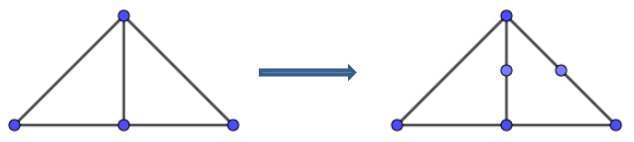
\includegraphics[scale=0.6]{img/suddivisione.PNG}
    \caption{esempio suddivisione}
\end{figure}
\begin{definizione}[Contrazione]
    Operazione inversa della suddivisione, consiste nell'contrarre un arco avente un endpoint di grado 2.
\end{definizione}

\begin{definizione}[Grafi omeomorfi]
    Due grafi \(G_1,G_2\) si dicono topologicamente equivalenti o omeomorfi se possono essere trasformati l'uno nell'altro attraverso operazioni di suddivisione o contrazione degli archi.
    \\ Denotiamo l'insieme dei grafi omeomorfi a \(G\) con \(TG\).
\end{definizione}

\begin{definizione}[Minore]
    \(H\) è detto minore di \(G\) se \(H\) è un grafo ottenuto da \(G\) tramite una sequenza di operazioni di rimozione di archi, vertici o contrazione di archi.
\end{definizione}

\begin{definizione}[Facial walk]
    Sia \(G\) grafo, \(G^\psi\) una sua immersione nel piano. Un cammino chiuso \(C\) frontiera di una faccia \(F\) di \(G^\psi\) è detto facial walk di F.
\end{definizione}

\begin{definizione}[Grado di una faccia]
    Definaiamo \(\deg(F)\) grado di una faccia \(F\) come la lunghezza del suo facial walk.
\end{definizione}
\begin{definizione}[Grafo semplice]
    Grafo contentente un numero finito di nodi.
\end{definizione}
\begin{definizione}[Grafo planare]
    Un grafo non orientato \(G\) si dice planare se può essere rappresentato nel piano evitando che gli archi si intersechino (se non negli endpoint).
\end{definizione}
\subsection{Topologia}
\begin{definizione}[n-cella chiusa]
    Spazio topologico omeomorfo ad una palla chiusa n-dimensionale.
\end{definizione}
\begin{definizione}[Complesso cellulare (CW-complesso)]
    Spazio topologico ottenuto incollando tra loro un insieme di celle chiuse.
\end{definizione}
\begin{definizione}[Caratteristica di eulero]
    Sia \(\tau \subset \mathbb{R}^n\) un complesso cellulare composto da \(k_i\) i-celle \(i=0,\dots,n\). Definiamo caratteristica di eulero
    \begin{equation}
        \chi(\tau) = k_0 - k_1 + k_2 - \dots k_n = \sum_{i=0}^{n}{(-1)}^i k_i
    \end{equation}
\end{definizione}

\begin{definizione}[Cammini omotopi]
    Siano \(f,g \in \mathcal{C}^0(X;Y)\). Diciamo \(f\) e \(g\) omotope \(f \sim g\) se esiste \(H : X \times [0,1] \to Y\) t.c.
    \begin{equation}
        \forall x \in X \begin{cases}
            H(x,0)=f(x) \\
            H(x,1)=g(x)
        \end{cases}
    \end{equation}
    Informalmente questo vale se una mappa può essere “deformata con continutià” nell'altra.
\end{definizione}

\begin{definizione}[Spazi omotopicamente equivalenti]
    \(X,Y\) si dicono omotopicamente equivalenti (\(X\sim Y\)) se \(\exists f : X \to Y, g:Y \to X \) t.c.
    \begin{itemize}
        \item \(g \circ f \sim id_X\)
        \item \(f \circ g \sim id_Y\)
    \end{itemize}
    Informalmente \(X,Y\) saraano omotopicamente equivalenti se possono essere trasformati l'uno nell'altro con operazioni di deformazione.
\end{definizione}

\begin{lemma}[Omotopicamente invariante]\label{om-inv}
    La caratteristica di eulero è un omotopicamente invariante, ovvero
    \begin{equation}
        X \sim Y \Rightarrow \chi (X) = \chi (Y)
    \end{equation}
\end{lemma}

\begin{proposizione}[Invarianza topologica]\label{inv-top}
    La caratteristica di eulero è un invariante topologico, ovvero
    \begin{equation}
        X \simeq Y \Rightarrow \chi (X) = \chi (Y)
    \end{equation}
    diciamo che \(X \simeq Y\) se \(X\) e \(Y\) sono omeomorfi.
\end{proposizione}

\begin{lemma}
    Ogni poliedro semplice può essere identificato come un grafo planare usando i vertici del poliedro come vertici del grafo e gli spigoli del poliedro come archi del grafo.
\end{lemma}
\begin{proposizione}
    Sia \(\tau\) un poliedro semplice allora \(\chi(\tau)=2\)
    \begin{proof}
        Questo risultato segue direttamente dal lemma precedente e dal teorema \(\ref{formulaeulero}\).
    \end{proof}
\end{proposizione}



